\chapter{Analyse syntaxique du fichier }

\section{Grammaire utilisée}

La grammaire à pu être représentée par l'arbre suivant, sur un des exemples dans le sujet du projet : 
\begin{figure}[H]
\centering
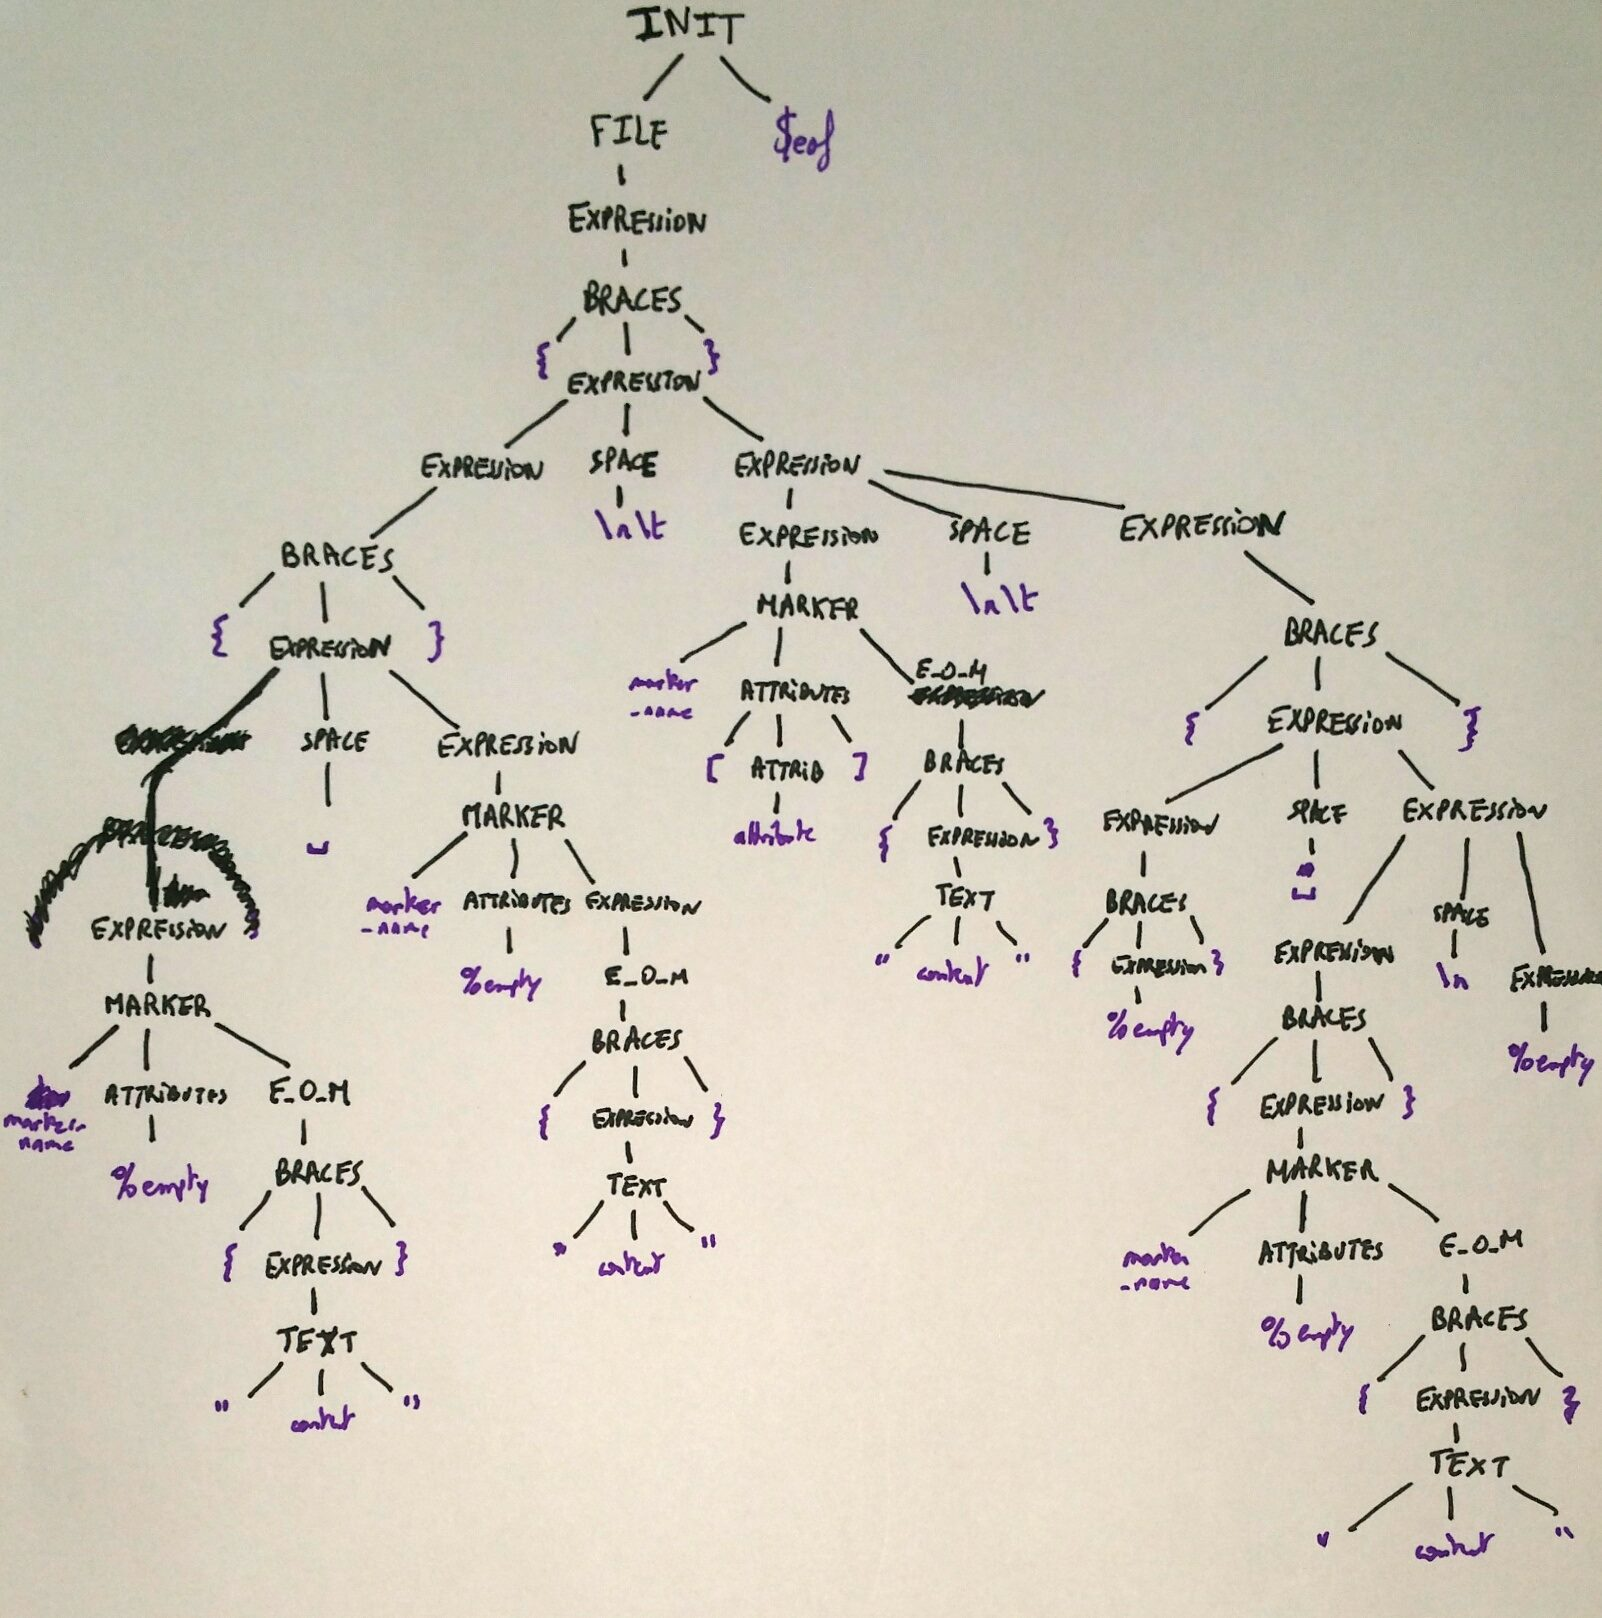
\includegraphics[scale=0.25]{Arbre.jpg}
\caption{}
\end{figure}

Le fichier lex main.l va servir d'analyseur syntaxique. Et va parser chaque mot du fichier donné pour ainsi print les balises en format adéquat HTML.\newline
La grammaire prend normalement en compte les "$\backslash$" Ainsi que les "$\backslash$ $\backslash$ " \newline
\newline


Nous l'avons ensuite créée sous la forme suivante :\newline
\newline

\begin{verbatim}
%token E_O_F TEXT_CONTENT ATTRIBUTE SPACE
%token XML_FREE_TEXT
%start init

%%

// Règle initiale

init 	: expr_set E_O_F
;

// Cas du fichier vide
// Puisque la balise <body> est posée, on suppose pouvoir
// mettre directement du texte

expr_set 	: expr_set SPACE expression 
    		| expression 						
    		| %empty 						
;

// Expressions principales

expression 	: marker 								
		   	| braces 								
		   	| text 									
;

// Balises

marker 	: XML_FREE_TEXT attributes end_of_marker	
;

// Attributs

attributes 	: '[' attrib ']'					 	
	   		| %empty								
;

attrib 	: attrib ',' attrib_alt 					
		| attrib ',' SPACE attrib_alt 				
       	| attrib_alt								
;

attrib_alt	: text_content '=' text 				
;

// Fin de balise
end_of_marker 	: braces 							
	      		| '/'								
;

// Accolades isolées (indépendantes d'une balise)
// Suffit par réductabilité d'expression

braces 	: '{' expr_set '}'							
;

// Texte simple

text 	: '"' text_content '"'
;

text_content 	: TEXT_CONTENT 						
				| XML_FREE_TEXT						
;
\end{verbatim}